\chapter{Elementary Probability Theory}

Probability theory is a mathematical formalism to describe and quantify uncertainty.
\\
\\ Uses of probability include examples such as:
\begin{itemize}
	\item Finding distribution of runtimes \& memory usage for software.
	\item Response times for database queries.
	\item Failure rate of components in a datacenter.
\end{itemize}

\section{Sample Spaces and Events}
\begin{definitionbox}{Sample Space}
	The set of all possible outcomes of a random experiment. The set is usually denoted with set notation, and can be finite, countably or uncountably infinite.
	\\
	\\ For example:
	\begin{center}
		\begin{tabular}{l l}
			\textbf{Experiment}  & \textbf{Sample Space}                                                \\
			\hline
			Coin Toss            & $S = \{Heads, Tails\}$                                               \\
			6-Sided Dice Roll    & $S = \{1,2,3,4,5,6\}$                                                \\
			2 Coin Tosses        & $S = \{(H,H), (H,T), (T,H), (T,T)\}$                                 \\
			Choice of Odd number & $S = \{ x \in \mathbb{N} | \exists y \in \mathbb{N}.[2y + 1 = x] \}$
		\end{tabular}
	\end{center}
\end{definitionbox}
\begin{definitionbox}{Event}
	Any subset of the sample space $E \subseteq S$ (a set of possible outcomes).
	\begin{itemize}
        \bullpara{null event($\emptyset$)}{Empty event, can be used for impossible events.}
		\bullpara{universal event ($S$)}{Event contains entire sample space and is therefore certain.}
		\bullpara{elementary events}{Singleton subsets of the sample space (contain one element).}
    \end{itemize}
    For example:
    \begin{center}
        \begin{tabular}{l l l}
            \textbf{Event}             & \textbf{Set of Event} & \textbf{Sample Space}                \\
            \hline
            6-Sided Dice Rolls 1       & $E = \{1\}$           & $S = \{1,2,3,4,5,6\}$                \\
            6-Sided Dice Rolls Even    & $E = \{2,4,6\}$       & $S = \{1,2,3,4,5,6\}$                \\
            6-Sided Dice Rolls 7       & $E = \emptyset$       & $S = \{1,2,3,4,5,6\}$                \\
			2 Coin toss get 2 Tails    & $E = \{(T,T)\}$       & $S = \{(H,H), (H,T), (T,H), (T,T)\}$ \\
			Random Natural Number is 4 & $E = \{4\}$           & $S = \mathbb{N}$                     \\
		\end{tabular}
	\end{center}
\end{definitionbox}
\begin{center}
    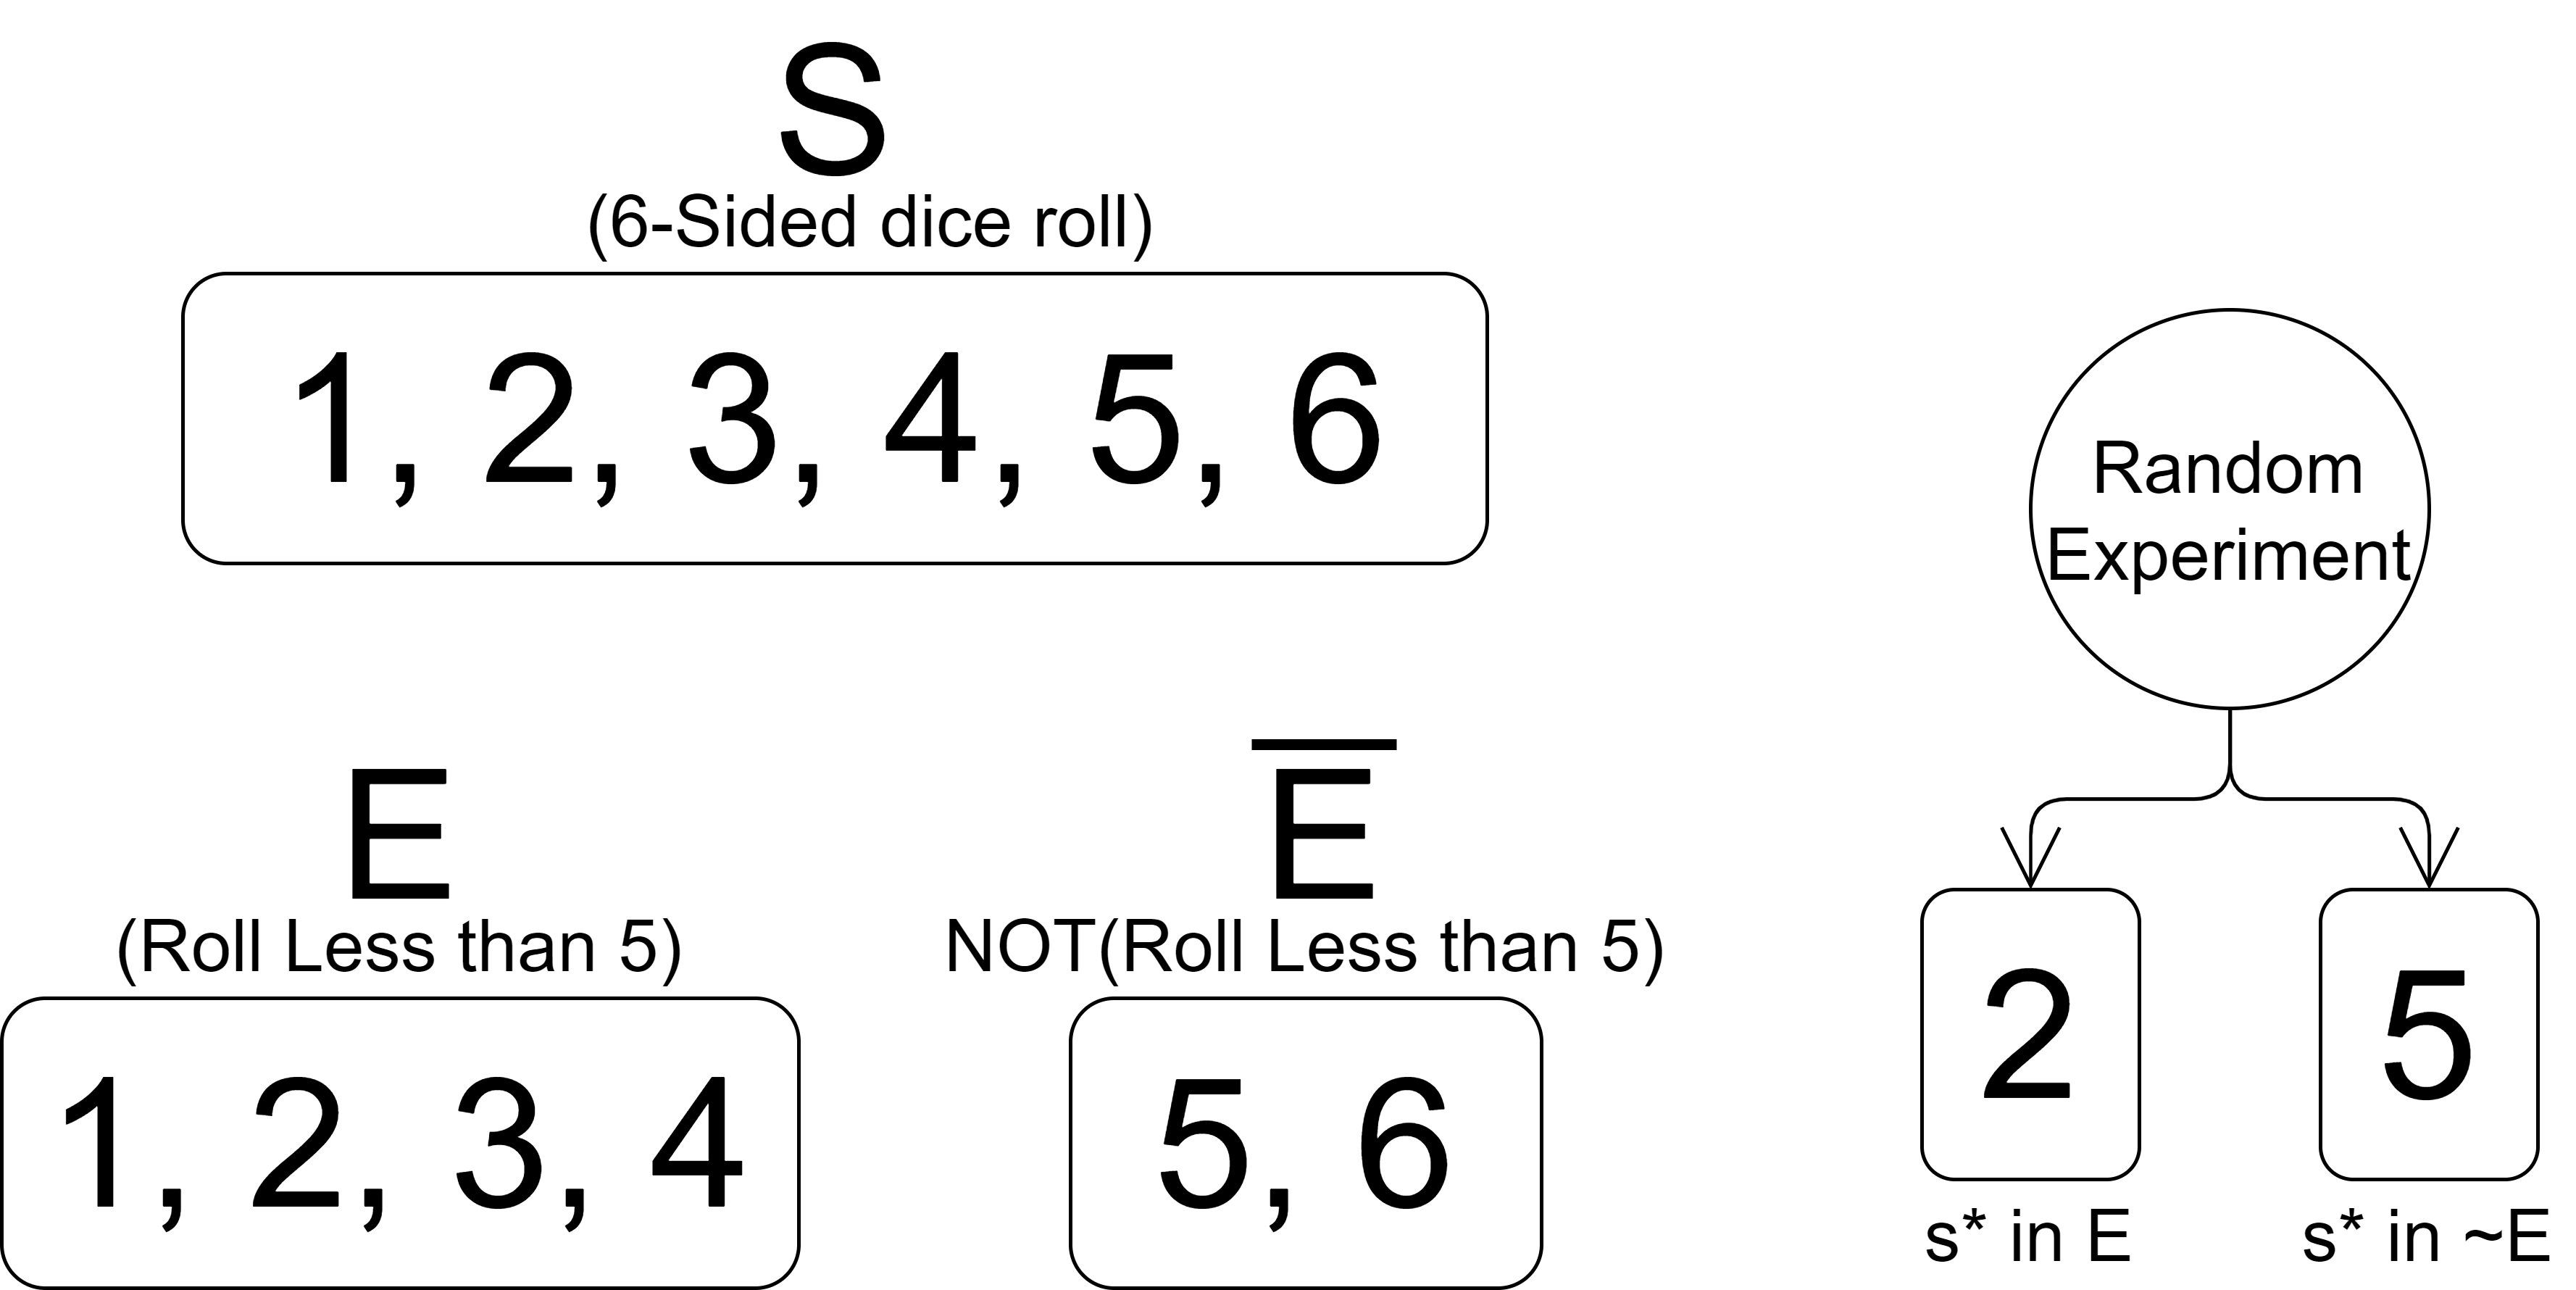
\includegraphics[width=0.7\textwidth]{elementary_probability_theory/images/experiment.drawio.png}
\end{center}
\begin{itemize}
	\item If we perform a random experiment with outcome $S* \in S$. If $s* \in E$, then event $E$ has occurred.
	\item If $E$ has not occurred ($s* \not\in E$) then $s* \in \overline{E}$.
	\item The set $\{s*\}$ is an elementary event.
	\item Null event $\emptyset$ never occurs, the universal event $S$ always occurs.
\end{itemize}
\subsection{Set Operations on Events}
\begin{itemize}
	\bullpara{Union / Or}{
		\[\bigcup_iE_i = \{s \in S | \exists i .[s \in E_i] \} \]
		Occurs if at least one of the events $E_i$ has occurred (has union of event sets).
		\\
		\\ If 4 is rolled on a 6-sided dice, then union of (is 3) and (is 4) occurred.
	}
	\bullpara{Intersection / And}{
		\[\bigcap_iE_i = \{s \in S | \forall i. [s \in E_i]\}\]
		Occurs if all the events $E_i$ occur.
		\\
		\\ If 4 is rolled on a 6-sided dice, the intersection of (is even) and (is 4) occurred.
	}
	\bullpara{Mutual Exlusion}{
		\[E_1 \cap E_2 = \emptyset\]
		If sets are disjoint, then they are mutually exclusive (cannot occur simultaneously).
		\\
		\\ For a 6-sided dice the events (is 4) and (is 6) are mutually exclusive.
	}
\end{itemize}

\subsection{Probability}
When determining the probability of every subset $E \subseteq S$ occurring:
\begin{itemize}
	\bullpara{$S$ is Finite}{Can easily assign probabilites.}
	\bullpara{$S$ is countable}{Can assign probabilites.}
	\bullpara{$S$ is uncountably infinite}{
        \\ Can initially assign some collection of subsets probabilities, but it then becomes impossible to define probabilities on reamining subsets.
		\\
		\\ Cannot make probabilities sum to $1$ with reasonably axioms.
    }
\end{itemize}
For this reason when defining a probability function on sample space $S$, we must define the collection of subsets we will measure.
\\
\\ The subsets are referred to as $\mathcal{F}$ and must be:
\begin{enumerate}
	\item nonempty ($S \in \mathcal{F}$)
	\item closed under complements $E \in \mathcal{F} \Rightarrow \overline{E} \in \mathcal{F}$
	\item closed under countable union $E_1, E_2, \dots \in \mathcal{F} \Rightarrow \bigcup_iE_i \in \mathcal{F}$
\end{enumerate}
A collection of sets is known as $\sigma$-algebra.
\begin{definitionbox}{Probability Measure}
	A function $P: \mathcal{F} \to [0,1]$ on the pair $(S,\mathcal{F})$ such that:
	\begin{center}
		\begin{tabular}{l l}
			Axiom 1. & $\forall E \in \mathcal{F}.[0 \leq P(E) \leq 1]$                                                                   \\
			Axiom 2. & $P(S) = 1$                                                                                                         \\
			Axiom 3. & Countably additive, for \textbf{disjoint} sets $E_1, E_2, \dots \in \mathcal{F}$: $P(\bigcup_iE_i) = \sum_iP(E_i)$
		\end{tabular}
	\end{center}
	$P(E)$ provides the probability (between 0 and 1 inclusive) that a given event occurs.
\end{definitionbox}

From the axioms satisfied by a \keyword{probability measure} we can derive that:
\begin{enumerate}
    \item $P(\overline{E}) = 1 - P(E)$
    \item $P(\emptyset) = 0$
    \item For any events $E_1$ and $E_2$: $P(E_1 \cup E_2) = P(E_1) + P(E_2) - P(E_1 \cap E_2)$
\end{enumerate}

\section{Interpretations of Probability}
\subsection{Classical Interpretation}

Given $S$ is finite and the \keyword{elementary events} are equally likely:
\[P(E) = \cfrac{|E|}{|S|}\]
We can also extend this \keyword{uniform probability distribution} to infinite spaces by considering measures such as area, mass or volume.
\begin{center}
    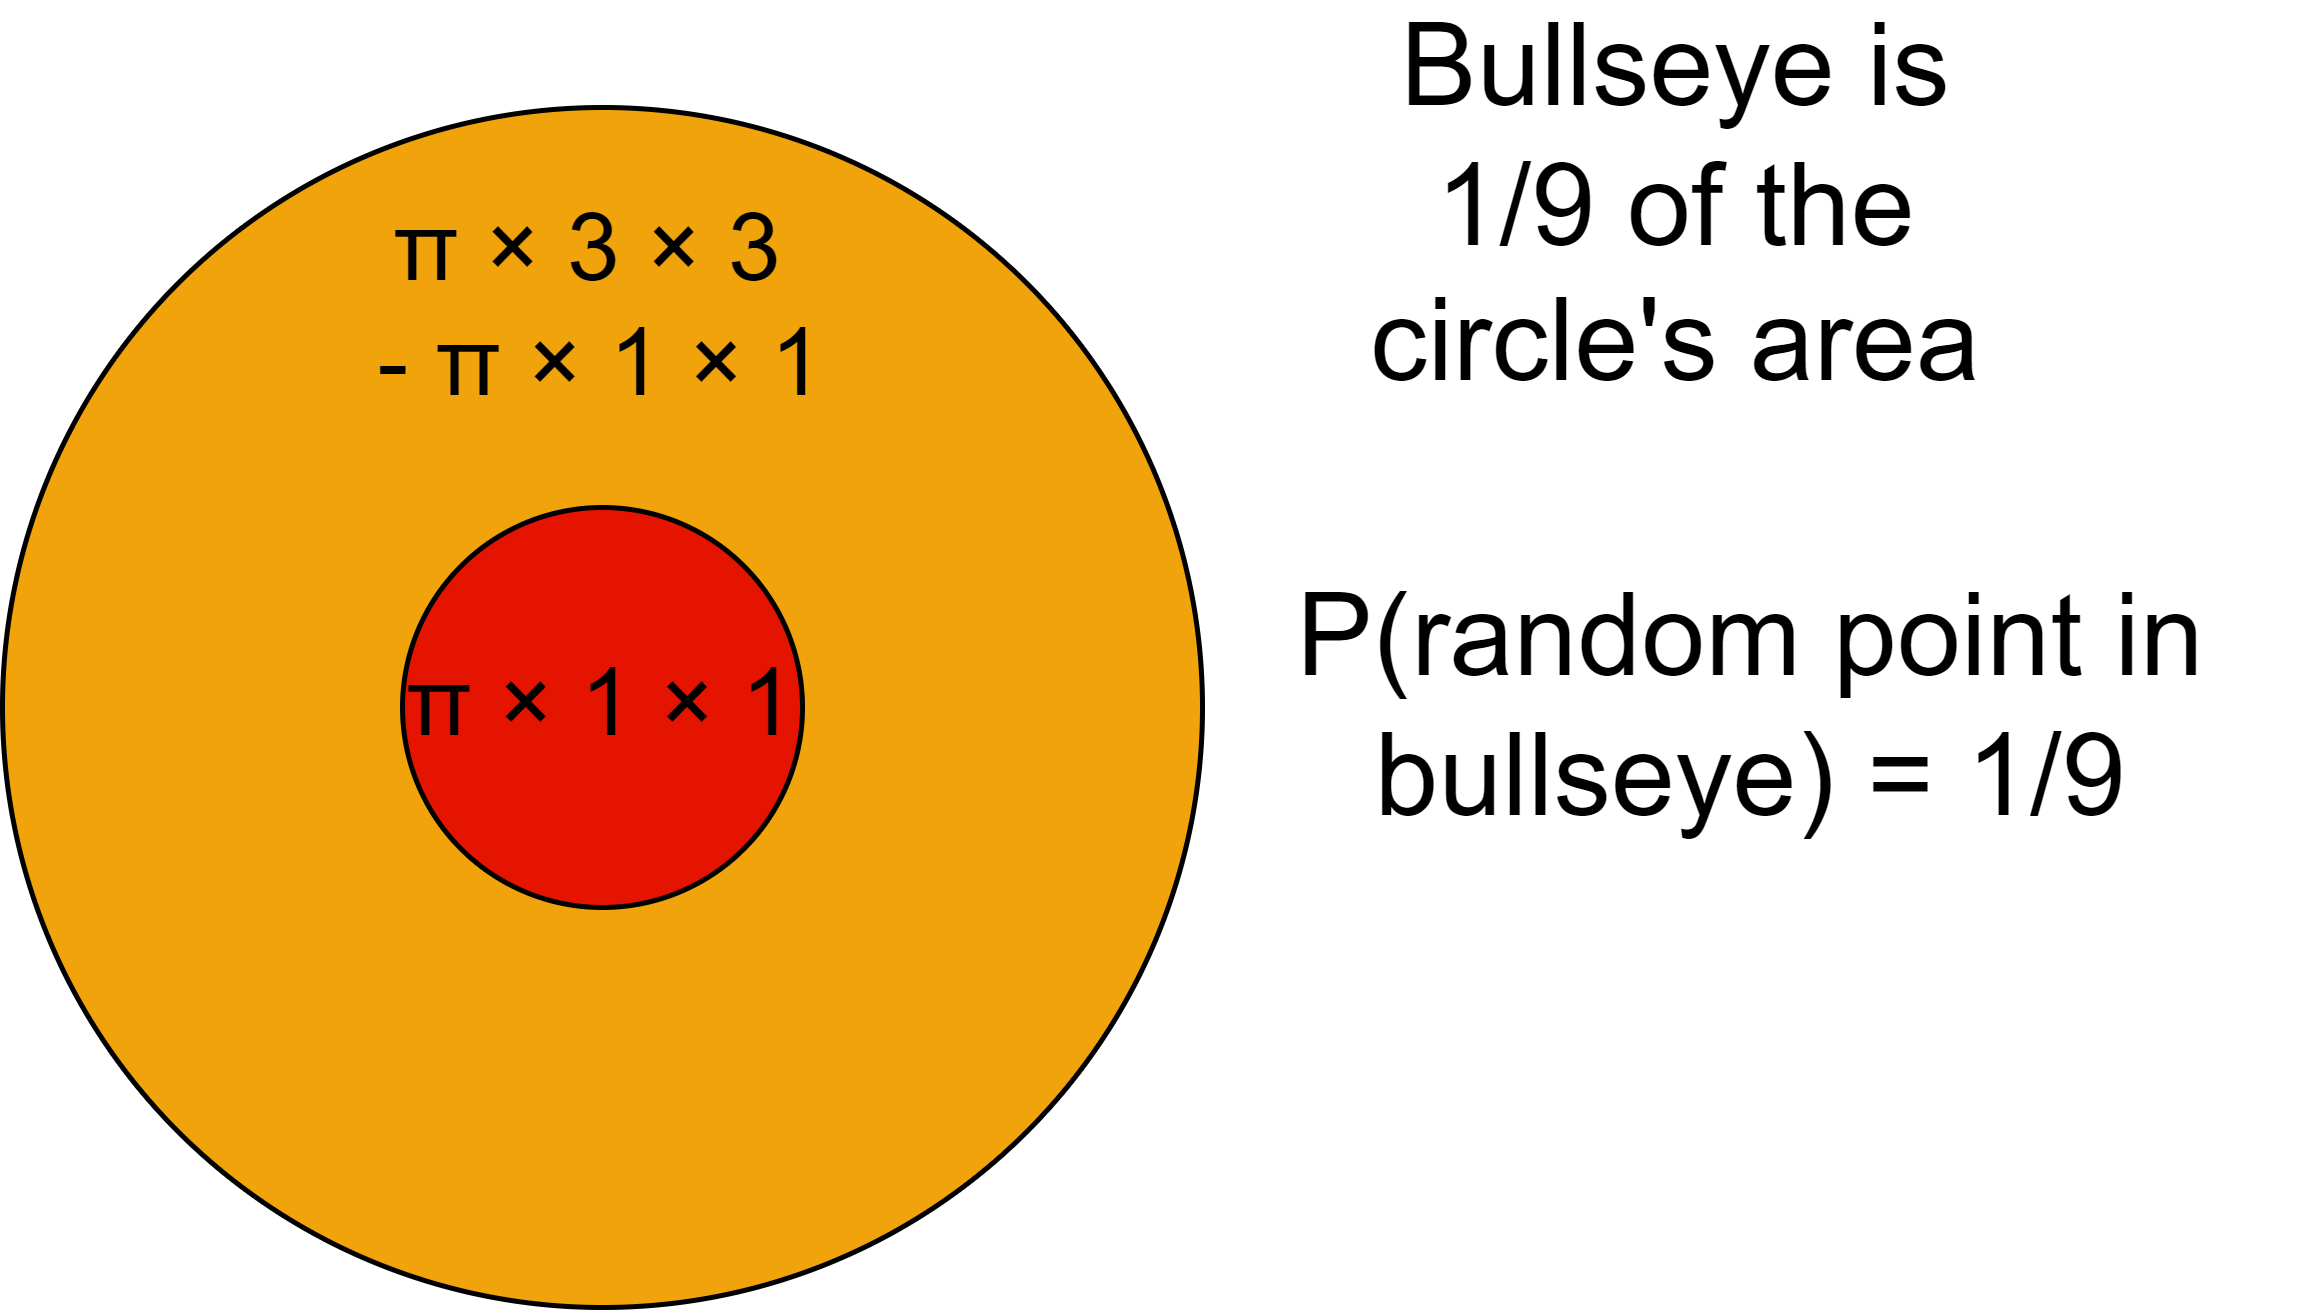
\includegraphics[width=.5\textwidth]{elementary_probability_theory/images/uniform area.drawio.png}
\end{center}

\subsection{Frequentist Interpretation}
Through repeated observations of identical random experiments in which $E$ can occur, the proportion of experiments where $E$ occurs tends towards the probability of $E$.
\\
\\ At an infinite number experiments, the proportion of occurrences of $E$ is equal to $P(E)$.
\begin{sidenotebox}{Central Limit Theorem}
	This can also be considered in terms of \keyword{central limit theorem}, where the greater the sample size taken from some distribution (with defined mean $\mu$), the closer the mean of the sample to the distribution's mean. (more readings results in less variance in the sample means as they converge on the distribution's mean)
\end{sidenotebox}

\subsection{Subjective Interpretation}
Probability is the degree of belief held by an individual.
\\
\\ For example if gambling: \begin{tabular}{l l}
	Option 1: $E$ occurs win $\pounds 1$, $\overline{E}$ occurs win $\pounds 0$ \\
	Option 2: Regardless of outcome get $\pounds P(E)$                   \\
\end{tabular}.
\\
\\ Either outcome, the gambler receives $\pounds P(E)$. The value of $P(E)$ is the value for which the individual is indifferent about the choice between option 1 or 2. It is the \keyword{individuals probability} of event $E$ occurring.


\section{Joint Events and Conditional Probability}
We commonly need to consider \keyword{Join Events} (where two events occur at the same time).
\begin{definitionbox}{Independent Events}
    Two events are independent if the occurence of one does not affect the other. Given $E_1$ and $E_2$ are independent:
    \[E_1 \ and \ E_2 \ independent \Leftrightarrow P(E_1 \ occurrs \ and \ E_2 \ occurs) = P(E_1) \times P(E_2)\]
    More generally, the set of events $\{E_1, E_2, \dots\}$ are independent if for any finite subset $\{E_{i_1}, E_{i_2}, \dots, E_{i_n}\}$:
    \[p(\bigcap_{j=1}^{n}E_{i_j}) = \prod_{j=1}^n P(E_{i_j}) \]
    If $E_1$ and $E_2$ are independent, then so are $\overline{E_1}$ and $E_2$.
    \\
    \\For example with a coin toss, subsequent coin tosses do not effect the next coin toss's probability of heads.
\end{definitionbox}

We can show that if $E_1$ and $E_2$ are independent, so are $\overline{E_1}$ and $E_2$:
\begin{proof}
	\proofstep{1}{$F = (E_1 \cap E_2) \cup (\overline{E_1} \cap E_2)$}{By set operations}
	\proofstep{2}{$P(E_2) = P(E_1 \cap E_2) + p(\overline{E_1} \cap E_2)$}{As \stepno{1} was a disjoint union, Axiom 3}
	\proofstep{3}{$P(\overline{E_1} \cap E_2) = P(E_2) - P(E_1 \cap E_2)$}{}
	\proofstep{4}{$P(\overline{E_1} \cap E_2) = P(E_2) - P(E_1) \times P(E_2)$}{}
	\proofstep{5}{$P(\overline{E_1} \cap E_2) = P(E_2) \times (1 - P(E_1)$}{}
	\proofstep{6}{$P(\overline{E_1} \cap E_2) = P(E_2) \times P(\overline{E_1})$}{By $P(\overline{E}) = 1 - P(E)$}
\end{proof}
We can show that $P(E_1 \cup E_2) = P(E_1) + P(E_2) - P(E_1 \cap E_2)$:
\begin{proof}
	\proofstep{1}{$E_1 \cup E_2 = E_1 \cup (E_2 \cap \overline{E_1})$}{From set theory}
	\proofstep{2}{$P(E_1 \cup E_2) = P(E_1 \cup (E_2 \cap \overline{E_1}))$}{By Axiom 3}
	\proofstep{3}{$P(E_1 \cup E_2) = P(E_1) + P(E_2 \cap \overline{E_1})$}{}
	\proofstep{4}{$P(E_2 \cap \overline{E_1}) = P(E_2) - P(E_1 \cap E_2)$}{By \stepno{3} of the previous proof and as $E_1$ and $E_2$ are independent}
\end{proof}
\begin{examplebox}{Dice for Money}
    We can construct a \keyword{Probability Table}:
    \begin{center}
        \begin{tabular}{c c c c c c c c c}
            \setlength{\tabcolsep}{3em}
                                       &                & \multicolumn{6}{c}{Dice} & \multirow{2}{*}{Totals}                                                                                          \\
                                       &                & 1                        & 2                       & 3               & 4               & 5               & 6                                \\
            \multirow{2}{*}{Coin}      & H              & $\sfrac{1}{12}$          & $\sfrac{1}{12}$         & $\sfrac{1}{12}$ & $\sfrac{1}{12}$ & $\sfrac{1}{12}$ & $\sfrac{1}{12}$ & $\sfrac{1}{2}$ \\
                                       & T              & $\sfrac{1}{12}$          & $\sfrac{1}{12}$         & $\sfrac{1}{12}$ & $\sfrac{1}{12}$ & $\sfrac{1}{12}$ & $\sfrac{1}{12}$ & $\sfrac{1}{2}$ \\
            \multicolumn{2}{c}{Totals} & $\sfrac{1}{6}$ & $\sfrac{1}{6}$           & $\sfrac{1}{6}$          & $\sfrac{1}{6}$  & $\sfrac{1}{6}$  & $\sfrac{1}{6}$  &                                  \\
        \end{tabular}
    \end{center}
    We can determine the probability of any event by summing the probabilities of elementary events represented by cells in the table.
    \\
    \\ $P({H})$ is called a \keyword{marginal probability}, as it the probability of one event occurring irrespective of the other (the dice in this case).
    \\
    \\ $P({(H,3)})$ is called a \keyword{joint probability} as it involves both events (dice roll and the coin toss).    
\end{examplebox}

\begin{examplebox}{Roll of the Die}
    A crooked die (called a top) has the same faces on either side.
    \\
    \\ We flip the coin, then if it is heads we use the normal die, else we use the top.
    \begin{center}
        \begin{tabular}{c c c c c c c c c}
            \setlength{\tabcolsep}{3em}
                                    &                & \multicolumn{6}{c}{Dice} & \multirow{2}{*}{Totals}                                                                                          \\
                                    &                & 1                        & 2                       & 3               & 4               & 5               & 6               &                \\
            \multirow{2}{*}{Coin}      & H              & $\sfrac{1}{12}$          & $\sfrac{1}{12}$         & $\sfrac{1}{12}$ & $\sfrac{1}{12}$ & $\sfrac{1}{12}$ & $\sfrac{1}{12}$ & $\sfrac{1}{2}$ \\
                                    & T              & $\sfrac{1}{6}$           & $0$                     & $\sfrac{1}{6}$  & $0$             & $\sfrac{1}{6}$  & $0$             & $\sfrac{1}{2}$ \\
            \multicolumn{2}{c}{Totals} & $\sfrac{1}{4}$ & $\sfrac{1}{12}$          & $\sfrac{1}{4}$          & $\sfrac{1}{12}$ & $\sfrac{1}{4}$  & $\sfrac{1}{12}$ &                                  \\
        \end{tabular}
    \end{center}
    We can now see that $P(\{(H,3)\}) \neq P(\{H\}) \times P(\{3\})$ and hence they are dependent, as the dice roll depends on the coin toss.
\end{examplebox}

\section{Conditional Probability}
For two events $E$ and $F$ in \keyword{sample space} $S$, where $P(F) \neq 0$:
\[P(E|F) = \cfrac{P(E \cap F)}{P(F)}\]
Probability of $E$ given $F$ is the probability of both occurring over the probability of $F$.
\begin{sidenotebox}{Independence}
    If $E$ and $F$ are independent:
    \[P(E|F) = \cfrac{P(E \cap F)}{P(F)} = \cfrac{P(E) \times P(F)}{P(F)} = P(E)\]
\end{sidenotebox}
\begin{definitionbox}{Conditional Independence}
	$P(\bullet | F)$ defines a probability measure obeying the axioms of probability on set $F$ (When have just reduced $S$ to $F$).
	\\
	\\ Three events $E_1, E_2, F$ are conditionally independent if and only if:
	\[P(E_1 \cap E_2|F) = P(E_1|F) \times P(E_2|F)\]
\end{definitionbox}

\begin{examplebox}
    What is the probability the dice rolls a $3$ given the dice rolls an odd number?
    \tcblower
    \[P(\{3\}|\{1,3,5\}) = \cfrac{P(\{3\} \cap \{1,3,5\})}{P(\{1,3,5\})} = \cfrac{P(\{3\})}{P(\{1,3,5\})} = \cfrac{\sfrac{1}{6}}{\sfrac{1}{2}} = \cfrac{1}{3}\]
\end{examplebox}
    
\begin{examplebox}{Go big or go home!}
Throw a die from each hand. What is the probability the die thrown from the left is larger than the die thrown from the right.
\tcblower
The sample space is:
\[S = \begin{Bmatrix}
		(1,1),(1,2),(1,3),(1,4),(1,5),(1,6), \\
        (2,1),(2,2),(2,3),(2,4),(2,5),(2,6), \\
        (3,1),(3,2),(3,3),(3,4),(3,5),(3,6), \\
		(4,1),(4,2),(4,3),(4,4),(4,5),(4,6), \\
        (5,1),(5,2),(5,3),(5,4),(5,5),(5,6), \\
        (6,1),(6,2),(6,3),(6,4),(6,5),(6,6)  \\
	\end{Bmatrix}\]
We want the event such that the left value of the pair is larger.
\\
\\ For value $1$ there are $0$ possible, for $2$ there is $1$ and so on.
\[(1:0),(2:1),(3:2),(4:3),(5:4),(6:5)\]
Hence there are $0 + 1 + 2 + 3 + 4 + 5 = 15$ possible pairs with the left larger than the right.
\[P(E) = \cfrac{15}{36} = \cfrac{5}{12}\]
However if we know the left or right die, we can determine a new probability. For example if we know the left die is $4$ then we know there are $6$ pairs with the left as $4$, and $3$ of those pairs have a smaller right.
\[P(E|{4}) = \cfrac{3}{6} = \cfrac{1}{2}\]
\end{examplebox}    
\begin{definitionbox}{Bayes Theorem}
	For two events $E$ and $F$ we have:
	\[P(E \cap F) = P(F) \times P(E|F) = P(F) \times \cfrac{P(E \cap F)}{P(F)} = P(E) \times P(F|E) = P(E) \times \cfrac{P(E \cap F)}{P(E)}\]
	Hence we can deduce:
	\[P(E|F) = \cfrac{P(E) \times P(F|E)}{P(F)}\]
    \begin{center}
        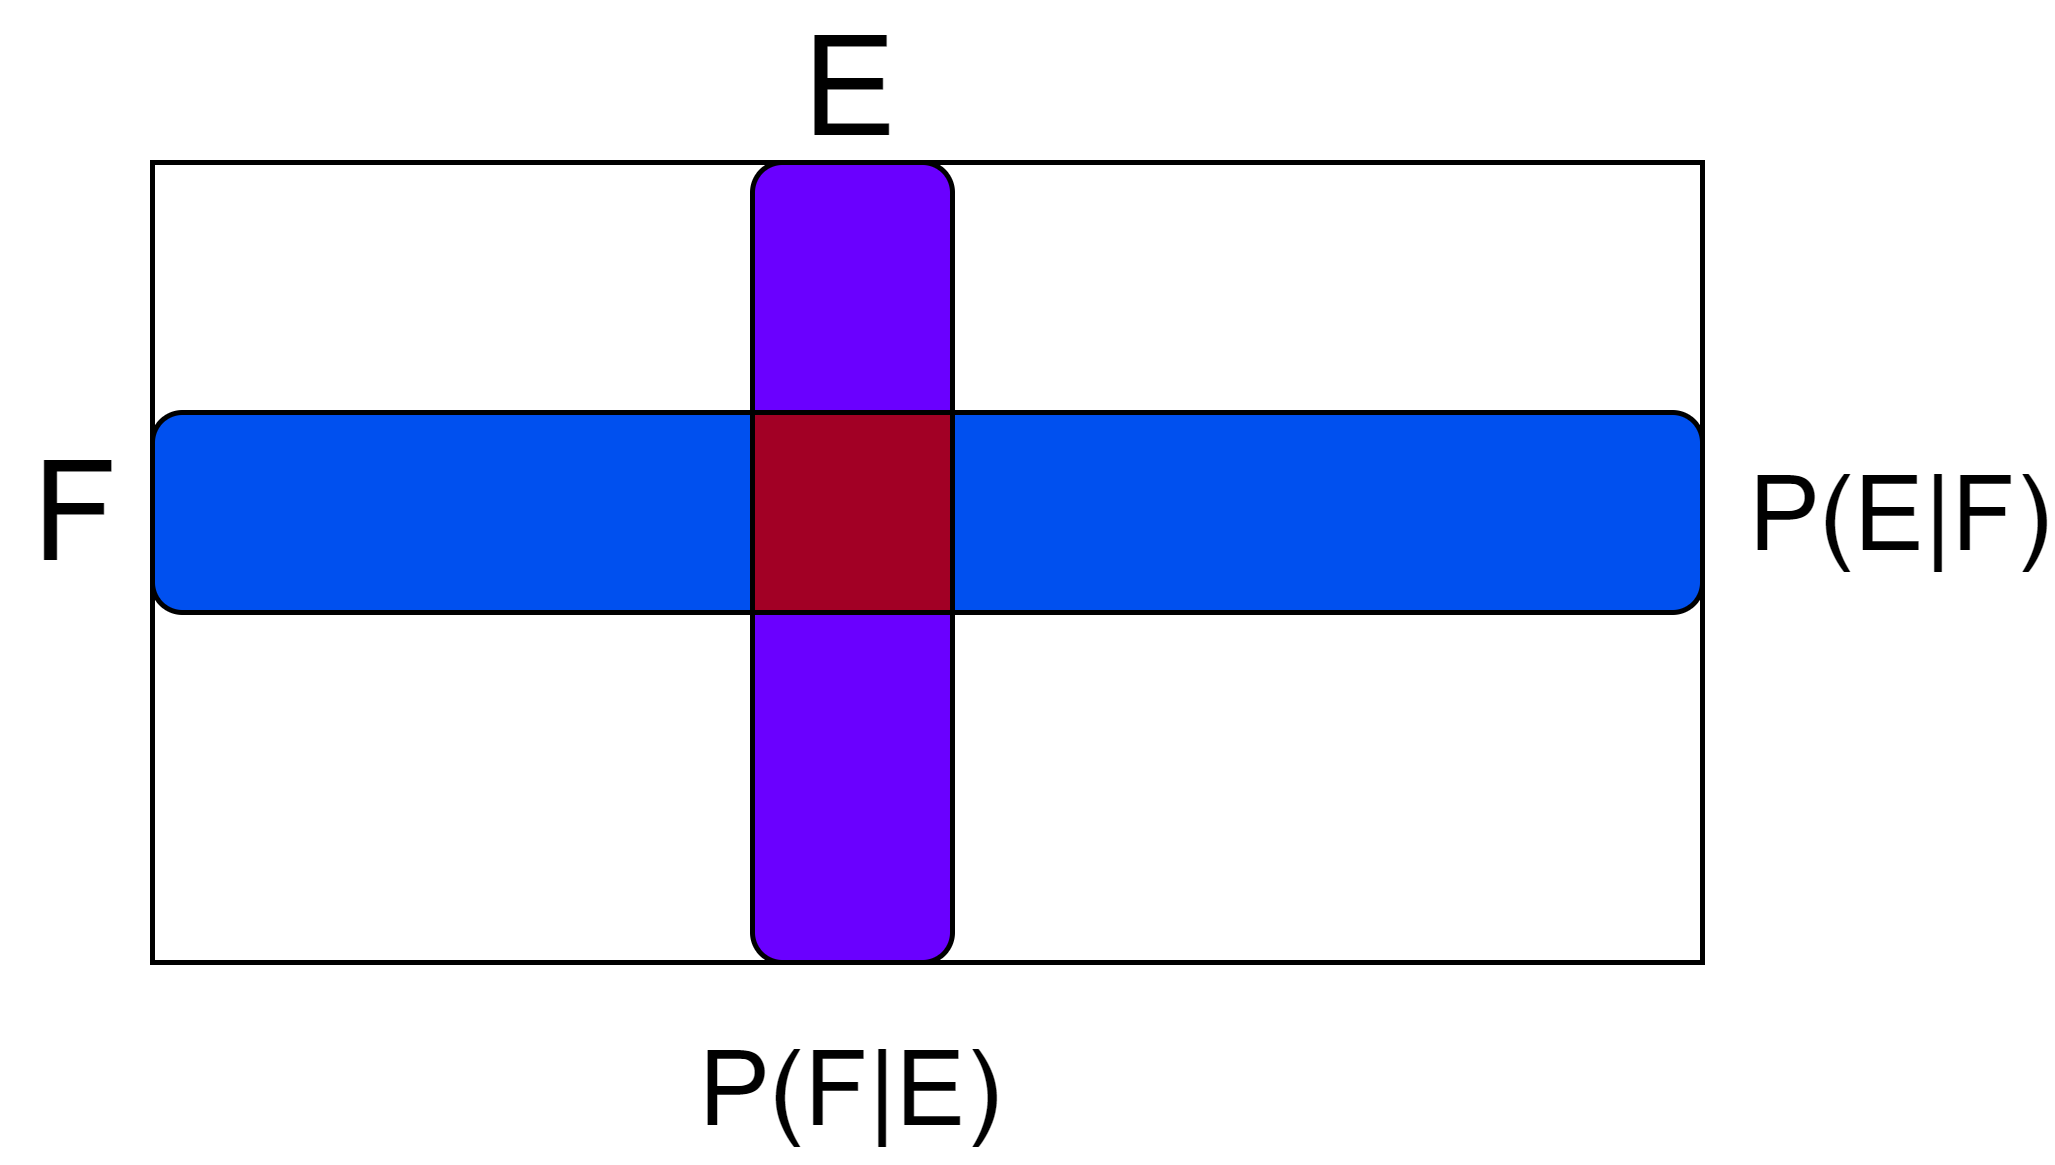
\includegraphics[width=.6\textwidth]{elementary_probability_theory/images/bayes theorem.drawio.png}
    \end{center}
\end{definitionbox}

\begin{definitionbox}{Partition Rule}
	Given a set of events $\{F_1, F_2, \dots\}$ which forms a partition of $S$ (disjoint sets that contain all of $F$).
	\\
	\\ For any event $E \subseteq S$:
	\[P(E) = \sum_iP(E|F_i) \times P(F_i)\]
	\centerimage{width=0.8\textwidth}{elementary_probability_theory/images/partition rule.drawio.png}
	Proof:
	\begin{proof}
		\proofstep{1}{$E = E \cap S = E \cap \bigcup_iF_i = \bigcup_i(E \cap F_i)$}{By set theory and disjointness of partitions.}
		\proofstep{2}{$P(E) = P(\bigcup_i(E \cap F_i))$}{}
		\proofstep{3}{$P(E) = \sum_i{P(E \cap F_i)}$}{By axiom 3 and disjointness of partitions.}
		\proofstep{4}{$P(E) = \sum_iP(E|F_i) \times P(F_i)$}{}
	\end{proof}
\end{definitionbox}

\begin{definitionbox}{Law of Total Probability}
    Given some event $E$ and events $\{F_1, F_2, \dots\}$:
    \[P(E) = \sum_i{P(E \cap F_i)}\]
    For example the 6-Sided dice, $E = {H}$ and $F = [\{1\},\{2\},\{3\},\{4\},\{5\},\{6\}]$, the marginal probability is the same as the sum of all cells in row $H$.
\end{definitionbox}

Using complement as a partition we can deduce that:
\[P(E) = P(E \cap F) + P(E \cap \overline{F})\]
\[P(E) = P(E|F) \times P(F) + P(E|\overline{F}) \times P(\overline{F})\]

\subsection{Terminology Recap}
\begin{itemize}
	\bullpara{Conditional Probabilities}{Of the form $P(E | F)$.}
	\bullpara{Joint Probabilities}{Of the form $P(E \cap F)$.}
	\bullpara{Marginal Probabilities}{Of the form $P(E)$.}
\end{itemize}
